\chapter{Influence of the number of triggered channels and parametrisation in Monte-Carlo.}
\label{appendix:ped_shift}

The correction applied function of the number of hits above 0.5 MIPs is only a global correction not an event to event basis correction. Thus a part of the effect remains in the time distribution or it may be another effect from the electronics that is not yet identified.\\
The effect can be clearly seen in figure \ref{fig:ped_shift_dist_para}. This effect has to be implemented in the simulation in order to match the timing distribution of electrons without also influencing the time distribution for muons. A parametrisation is thus implemented in the Monte-Carlo extracted from data. This parametrisation assumes the following, the effect is additional to the seen muon resolution giving then:
\begin{equation*}
	\text{RMS}_{\text{obs}}^2 = \text{RMS}_{\mu}^2 + \text{RMS}_{\text{effect}}^2
\end{equation*}
The $\text{RMS}_{\text{effect}}$ is extracted from data by fitting with a function of the following form:
\begin{equation*}
	f(t) = A \times e^{-\frac{(t-\mu_1)^2}{2(\sigma_1^2 + \sigma_{effect}^2)}} + B* \times e^{-\frac{(t-\mu_2)^2}{2(\sigma_2^2 + \sigma_{effect}^2)}} + C
\end{equation*}

\begin{figure}[htbp!]
	\begin{subfigure}[t]{0.49\textwidth}
		\centering
		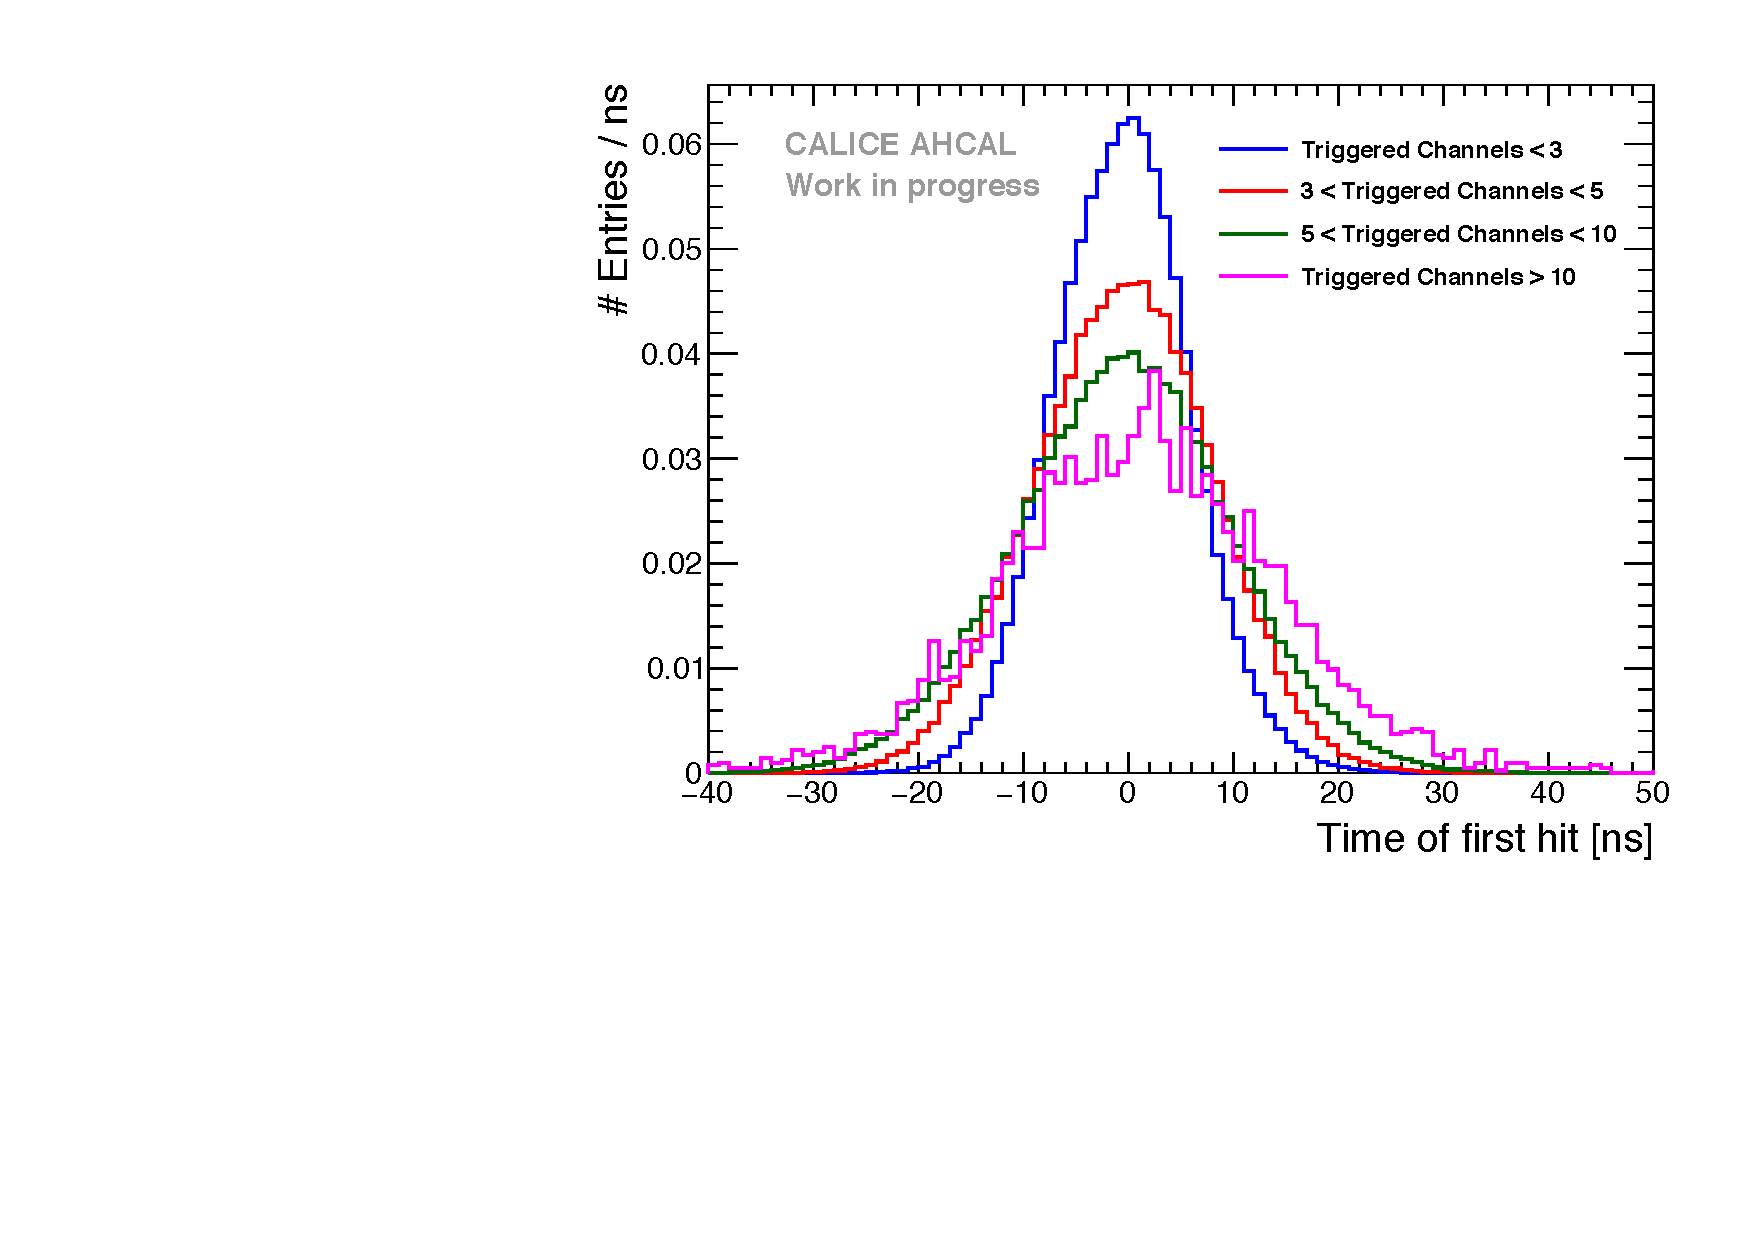
\includegraphics[width=1\linewidth]{chap5/fig_AHCAL_timing/Electrons/TimingHitsBins_20GeV.pdf}
		\caption{Time of the first hit distribution for different binning of number of triggered channels in a chip.} \label{fig:ped_shift_dist_para}
	\end{subfigure}
	\hfill
	\begin{subfigure}[t]{0.49\textwidth}
		\centering
		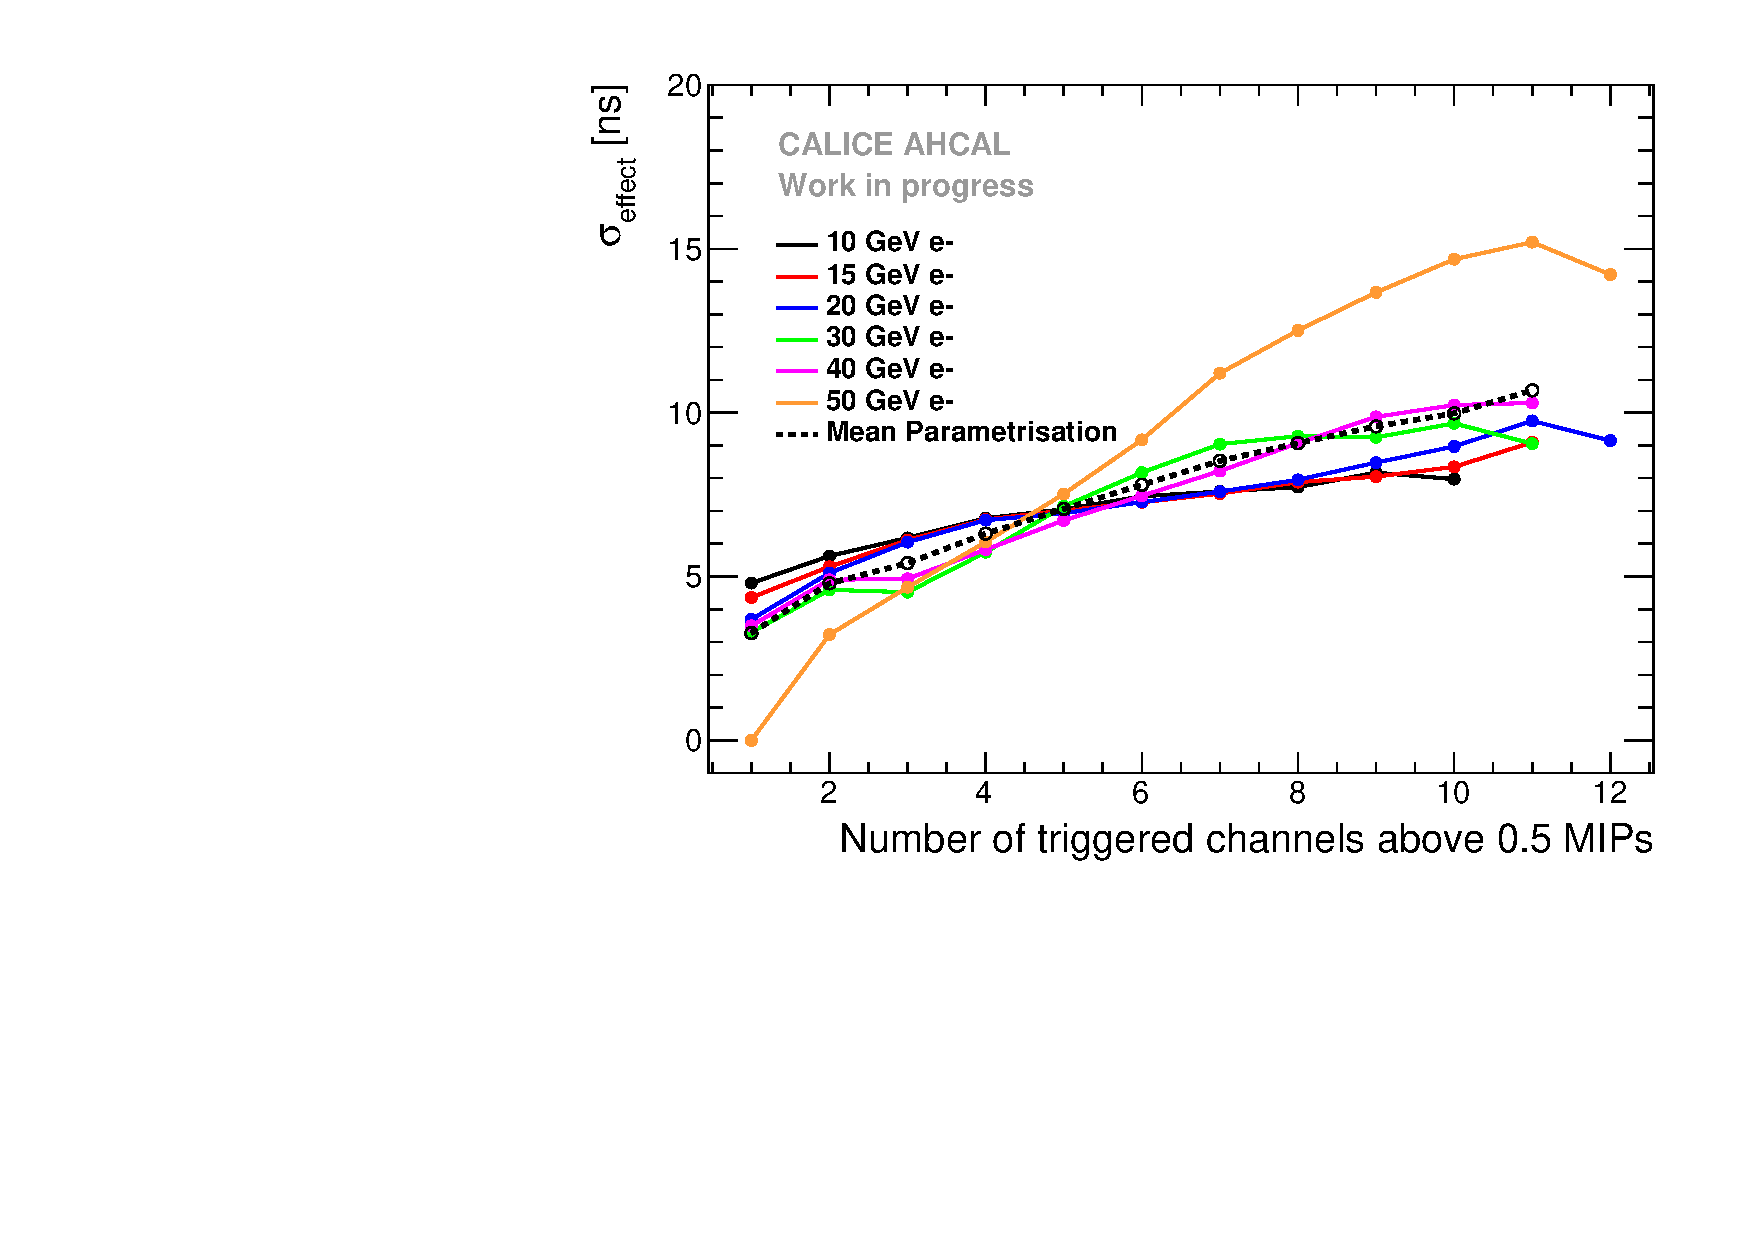
\includegraphics[width=1\linewidth]{chap5/fig_AHCAL_timing/Electrons/MeanParametrisation.pdf}
		\caption{$\sigma_{effect}$ extracted function of the number of triggered channels in a chip for each energies.} \label{fig:para_fit}
	\end{subfigure}
	\caption{\subref{fig:ped_shift_dist_para}) The distribution width is increasing with the number of triggered channels in a chip due to the remaining of the observed effect. \subref{fig:para_fit}) $\sigma_{effect}$ increases up to 12-15 ns with the number of triggered channels in a chip.}
\end{figure}

The parameters $\mu_1$, $\sigma_1$, $\mu_2$ and $\sigma_2$ are fixed from table \ref{table:time_res_sim}. By plotting $\sigma_{effect}$ extracted as a function of the number of triggered channels in a chip, one can extract the parametrisation of the effect. This is done for each electron energy point as shown in figure \ref{fig:para_fit}. One can observe that each parametrisation curve is slightly different for each energies. This may be due to the fact that each energy affects not exactly the same part of the detector. To accommodate this, a mean parametrisation is used in Monte-Carlo with the envelope used as uncertainty as shown in figure \ref{fig:mean_para}. Only points up to 10-11 number of channels are extracted from data. Above this, the value of $\sigma_{effect}$ is extrapolated. This should in principle have relatively a small effect for electrons as mainly 6-10 hits are expected per chip. But the effect may be relevant for pions.

\begin{figure}[htbp!]
	\centering
	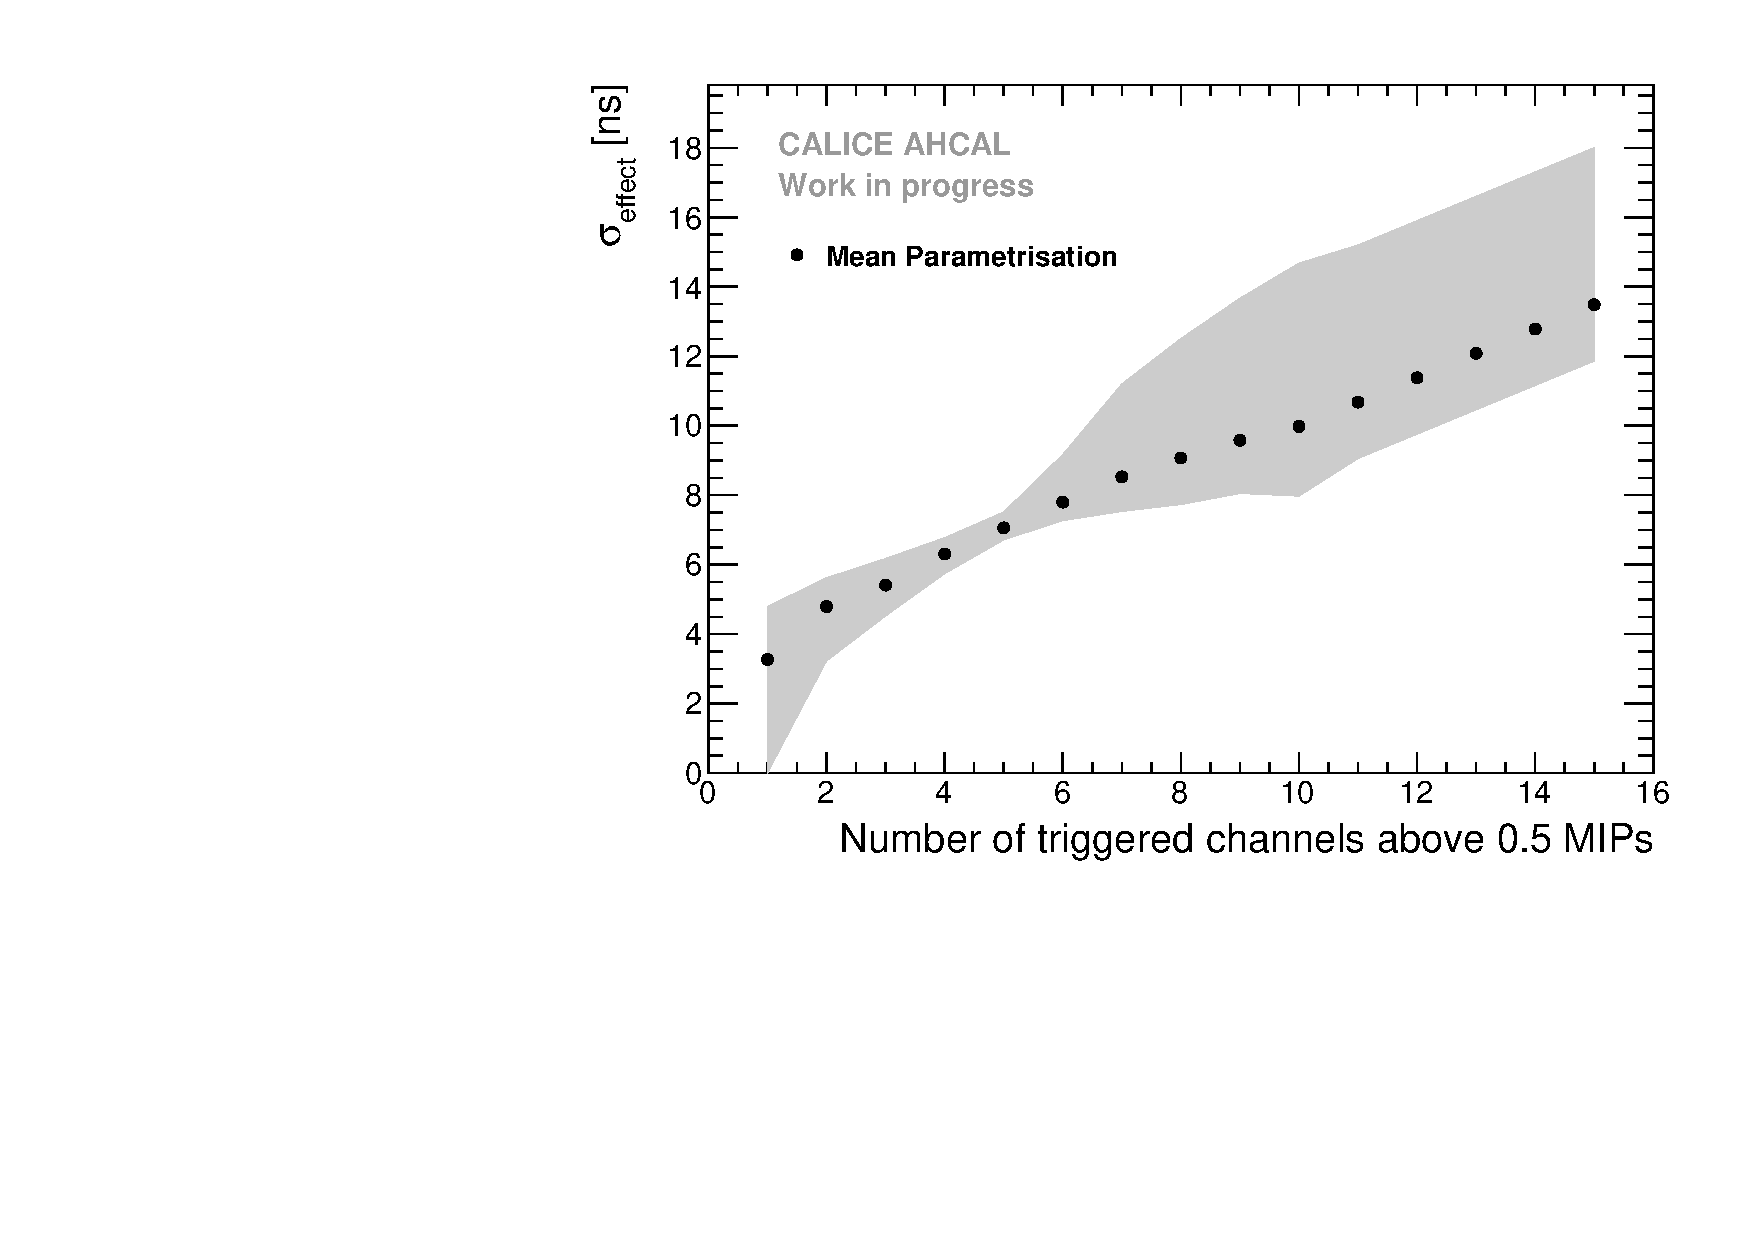
\includegraphics[width=0.7\linewidth]{chap5/fig_AHCAL_timing/Electrons/MeanParametrisationWithSystErrors.pdf}
	\caption{Mean parametrisation of $\sigma_{effect}$ as a function of number of triggered channels. The grey area represents the uncertainty.}
	\label{fig:mean_para}
\end{figure}
